\documentclass[12pt]{article}

\usepackage{times}
\usepackage{graphicx}
\usepackage{url}
\usepackage{amsmath}
\usepackage{float}

\setlength{\textwidth}{6.5in}
\setlength{\textheight}{8.9in}
\setlength{\oddsidemargin}{0.0in}
\setlength{\topmargin}{0.05in}
\setlength{\headheight}{-0.05in}
\setlength{\headsep}{0.0in}

\begin{document}

\begin{center}
{\bf CS 6300} \hfill {\large\bf HW6: Q Learning and Functional Approximation} \hfill {\bf Due March 7, 2017}
\end{center}

\noindent
Please use the \LaTeX\ template to produce your writeups. See the
Homework Assignments page on the class website for details.  Hand in
at: \url{https://webhandin.eng.utah.edu/index.php}.

\section{Approximate Q-Learning}

Consider the grid-world given below and Pacman who is trying to learn
the optimal policy.  If an action results in landing into one of the
shaded states the corresponding reward is awarded during that
transition.  All shaded states are terminal states, i.e., the MDP
terminates once arrived in a shaded state.  The other states have the
\textit{North, East, South, West} actions available, which
deterministically move Pacman to the corresponding neighboring state
(or have Pacman stay in place if the action tries to move out of the
grad).  Assume the discount factor $\gamma = 0.5$ and the Q-learning
rate $\alpha = 0.5$ for all calculations. Pacman starts in state (1,
3).

\begin{figure}[htb!]
\begin{center}
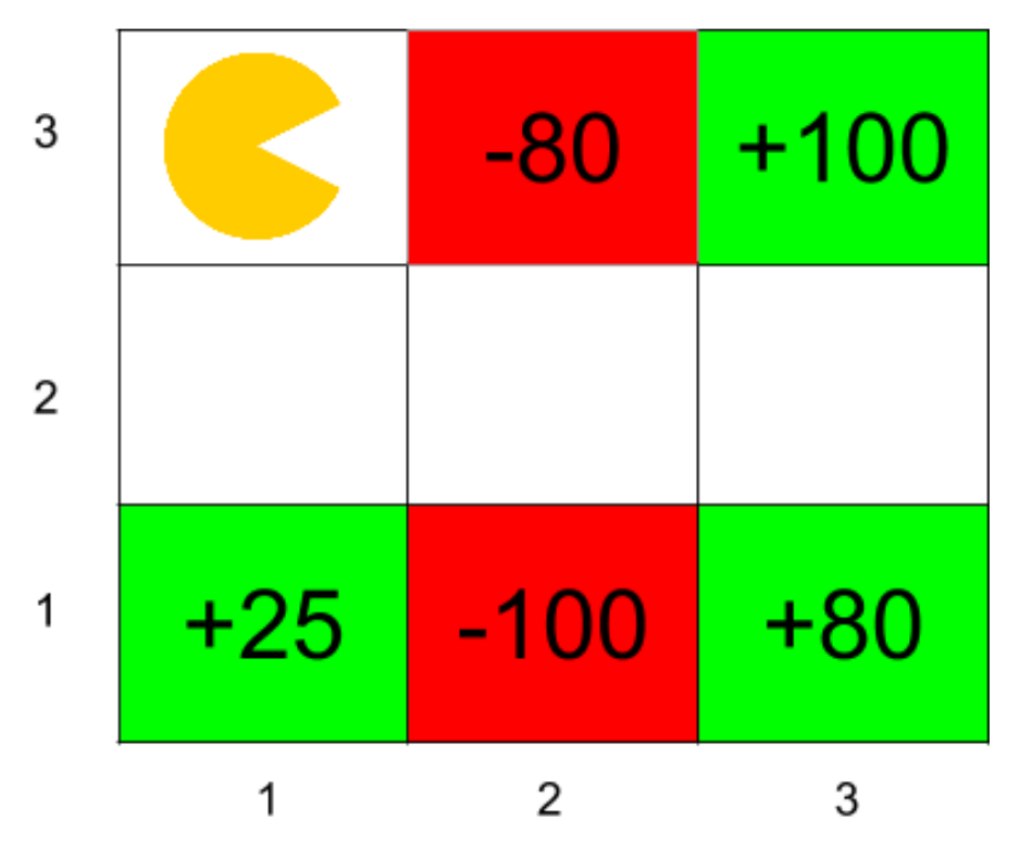
\includegraphics[height=4.5cm]{qlearn.png}
\end{center}
\end{figure}

\begin{enumerate}

\item What is the value of the optimal value function $V^*$ at the following states:
  
  \begin{center}\begin{tabular}{|l|l|} \hline
  \bf State  & \bf Optimal value \\ \hline
  $V^*(3,2)$ & 100\\
  $V^*(2,2)$ & 50\\
  $V^*(1,3)$ & 12.5\\ \hline
  \end{tabular}\end{center}

We want to calculate the optimal values from each of the states {\em onwards}, {\bf NOT} up until that point. The question states that the award is given {\em during transition into the state}, so we do not need to discount to get the award. Also, as we want to chose the maximum, we get the following:

\begin{itemize}
  \item $(3,2)$: Maximize to $100$ over $80$ since we want optimal
  \item $(2,2)$: Go to $100$ square, with a $1/2$ discount, $0 + \gamma(100) = 50$ to maximize
  \item $(1,3)$: Going to either $25$ or $100$ has the discounted reward of $12.5$
\end{itemize}

\item The agent starts from the top left corner and you are given the
  following episodes from runs of the agent through this
  grid-world. Each line in an Episode is a tuple containing $(s, a,
  s', r)$.

\begin{table}[htb!]
  \centering
\begin{tabular}{l|l|l}
Episode 1 & Episode 2 & Episode 3\\
\hline
(1,3), S, (1,2), 0 & (1,3), S, (1,2), 0 & (1,3), S, (1,2), 0 \\
(1,2), E, (2,2), 0 & (1,2), E, (2,2), 0 & (1,2), E, (2,2), 0 \\
(2,2), S, (2,1), -100 & (2,2), E, (3,2), 0 & (2,2), E, (3,2), 0 \\ 
  & (3,2), N, (3,3), +100 & (3,2), S, (3,1), +80 \\ 
 \hline
\end{tabular}
\end{table}

Using Q-Learning updates, what are the following Q-values after the
above three episodes:
  
  \begin{center}\begin{tabular}{|l|l|} \hline
  \bf Q State  & \bf Value \\ \hline
  $Q((3,2),N)$ & $50$\\
  $Q((1,2),S)$ & $0$\\
  $Q((2,2),E)$ & $12.5$\\ \hline
  \end{tabular}\end{center}

The $Q$-values can be found by the learning updates with the equation

\begin{align*}
Q(s,a) &= (1-\alpha)Q(s,a) + \alpha\left[ R(s,a,s^{\prime}) + \gamma\max_{a^{\prime}}Q(s^{\prime},a^{\prime})\right]
\intertext{We can do it for the first example, where we get $R(s,a,s^{\prime})$ as the reward is given on {\em transition}, giving}
Q((3,2),N) &= 0.5(0) + 0.5\left[ 100 + 0.5 \max_{a^{\prime}}(0)\right] = 50
\end{align*}

\item Consider a feature based representation of the Q-value function:

  \begin{equation*}
  Q_f(s,a)=w_1f_1(s)+w_2f_2(s)+w_3f_3(a)
  \end{equation*}

  \hfill $f_1(s):$ The x coordinate of the state \hfill $f_2(s):$ The y coordinate of the state \hfill \hfill\\\\
\centerline {$f_3(N)=1$, $f_3(S)=2$, $f_3(E)=3$, $f_3(W)=4$}
\\

  \begin{enumerate}

  \item Given that all $w_i$ are initially 0, what are their values
    after the first episode using approximate Q-learning weight
    updates.
  
  \begin{center}\begin{tabular}{|l|l|} \hline
  \bf Weight  & \bf Value \\ \hline
  $w_1$ & $-100$\\
  $w_2$ & $-100$\\
  $w_3$ & $-100$\\ \hline
  \end{tabular}\end{center}

  Using the equation for the $Q$-learning,

  \begin{align*}
    w_{i} &= w_{i} + \alpha\left[R(s,a,s^{\prime}) + \gamma\max_{a^{\prime}}Q(s^{\prime},a^{\prime}) - Q(s,a)\right]f_{i}(s,a)
    \intertext{In calculating this for the first weight, we get}
    w_{1} &= 0 + 0.5\left[ -100 + 0.5(0)\right]f_{1}\left((2,2)\right)\\
         &= 0 + 0.5\left[ -100 + 0.5(0)\right]2 = -100
    \end{align*}

    which when plugging in the values, we get $-100$ for each of the weights for the first episode.

  \item Assume the weight vector $w$ is equal to $(1, 1, 1)$.  What is
  the action prescribed by the Q-function in state $(2,2)$?

At $(2,2)$, the best action to maximize the value of $Q((2,2),a)$ is computed and is maximum for {\tt west} which gives $2+2+4$ which is a value of $8$.

  \end{enumerate}

\end{enumerate}

\clearpage

\section{Functional Approximation}

In this question, you will play a simplied version of blackjack where
the deck is infinite and the dealer always has a fixed count of 15.
The deck contains cards 2 through 10, J, Q, K, and A, each of which is
equally likely to appear when a card is drawn.  Each number card is
worth the number of points shown on it, the cards J, Q, and K are
worth 10 points, and A is worth 11.  At each turn, you may either {\it
  hit} or {\it stay}.

\begin{itemize}

\item If you choose to {\it hit}, you receive no immediate reward and
  are dealt an additional card.  

\item If you stay, you receive a reward of 0 if your current point
  total is exactly 15, +10 if it is higher than 15 but not higher than
  21, and -10 otherwise (i.e., lower than 15 or larger than 21).

\item After taking the {\it stay} action, the game enters a terminal
  state {\it end} and ends.

\item A total of 22 or higher is refered to as a {\it bust}; from a
  {\it bust}, you can only choose the action {\it stay}.

\end{itemize}

\noindent
As your state space you take the set $\{0,2,\ldots,21,bust,end\}$
indicating point totals.

\begin{enumerate}

\item Suppose you have performed $k$ iterations of value iteration.
  Compute $V_{k+1}(12)$ given the partial table below for $V_k(s)$.
  Give your answer in terms of the discount as a variable.

\begin{center}
\begin{tabular}{|r|r|} \hline
$s$  & $V_k(s)$\\ \hline
13   &   2     \\
14   &  10     \\
15   &  10     \\
16   &  10     \\
17   &  10     \\
18   &  10     \\
19   &  10     \\
20   &  10     \\
21   &  10     \\
bust & -10     \\
end  &  0      \\ \hline
\end{tabular}
\end{center}

Out of all of the cards, $(2-9)$ will take us to {\tt return} and $(10-A)$ will take us to {\tt bust}. This means that $V_{k+1}(12)$ is

\begin{align*}
   V_{k+1}(12) &= \frac{1}{13}\left[8(10\gamma) + 5(-10\gamma) \right]\\
              &= \frac{30}{13}\gamma
\end{align*}

\item You suspect that the cards do not actually appear with equal
  probability, and decide to use Q-learning instead of value
  iteration.  Given the partial table of initial Q-values below left,
  fill in the partial table of Q-values on the right after the episode
  center below occurs.  Assume $\alpha=0.5$ and $\gamma=1$.  The
  initial portion of the episode has been omitted.  Leave blank any
  values which Q-learning does not update.

\begin{center}
\begin{tabular}{ccc}
\begin{tabular}{|r|c|r|} \hline
$s$ & $a$  & $Q(s,a)$ \\ \hline
19  & hit  & -2 \\
19  & stay &  5 \\
20  & hit  & -4 \\
20  & stay &  7 \\
21  &  hit & -6 \\
21  & stay &  8 \\
bust& stay & -8 \\ \hline
\end{tabular} & 
\begin{tabular}{|c|c|c|c|} \hline
$s$ & $a$ & $r$ & $s'$ \\ \hline
19  & hit & 0   & 21   \\
21  & hit  & 0   & bust \\
bust& stay & -10 & end \\ \hline
\end{tabular} &
\begin{tabular}{|c|c|c|} \hline
$s$ & $a$  & $Q(s,a)$ \\ \hline
19  & hit  & $3$\\
19  & stay & \\
20  & hit  & \\
20  & stay & \\
21  & hit  & $-7$\\
21  & stay & \\
bust& stay & $-9$\\ \hline
\end{tabular}
\end{tabular}
\end{center}

These are calculated with the $Q$-learning equation, where the example for the first can be seen below

\begin{align*}
Q(19,hit) &= \frac{1}{2}(-2) + \frac{1}{2}\left[0 + 1\cdot\max (8, -6) \right]\\
          &= 3
\end{align*}

Where the others follow a similar nature.

\item Unhappy with your experience with basic Q-learning, you decide
  to featurize your Q-values.  Consider the two feature functions:

$$
f_1(s,a) = \left\{ \begin{array}{ll}
                  0  & a=stay \\
                  +1 & a=hit, s \geq 15 \\
                 -1  & a=hit, s < 15
                 \end{array} \right.
\quad \hbox{and} \quad
f_2(s,a) = \left\{ \begin{array}{ll}
                  0  & a=stay \\
                  +1 & a=hit, s \geq 18 \\
                 -1  & a=hit, s < 18
                 \end{array} \right.
$$

Which of the following partial policy tables may be represented by the
featurized Q-values unambiguously (without ties)?

\begin{center}
\begin{tabular}{ccccc}
\begin{tabular}{|c|c|} \hline
$s$ & $\pi(s)$ \\ \hline
14  & hit \\
15  & hit \\
16  & hit \\
17  & hit \\
18  & hit \\
19  & hit \\ \hline
\end{tabular} &
\begin{tabular}{|c|c|} \hline
$s$ & $\pi(s)$ \\ \hline
14  & stay \\
15  & hit \\
16  & hit \\
17  & hit \\
18  & stay \\
19  & stay \\ \hline
\end{tabular} &
\begin{tabular}{|c|c|} \hline
$s$ & $\pi(s)$ \\ \hline
14  & hit \\
15  & hit \\
16  & hit \\
17  & hit \\
18  & stay \\
19  & stay \\ \hline
\end{tabular} &
\begin{tabular}{|c|c|} \hline
$s$ & $\pi(s)$ \\ \hline
14  & hit \\
15  & hit \\
16  & hit \\
17  & hit \\
18  & hit \\
19  & stay \\ \hline
\end{tabular} &
\begin{tabular}{|c|c|} \hline
$s$ & $\pi(s)$ \\ \hline
14  & hit \\
15  & hit \\
16  & hit \\
17  & stay \\
18  & hit \\
19  & stay \\ \hline
\end{tabular} \\
(a) & (b) & (c) & (d) & (e)
\end{tabular}
\end{center}

The featurized $Q$-values can be calculated as $\omega_{1}f_{1}(s,a) + \omega_{2}f_{2}(s,a)$, where $\omega_{1}$ and $\omega_{2}$ are the weights for the features given above. Therefore, we need to calculate the $Q$-values to see if they hold. We get only $(c)$ as not having to break ties.

For example, we have in the table for $(a)$

\begin{table}[H]
\centering
\begin{tabular}{ccc}
\hline\hline
$Q(s,a)$ & $hit$ & $stay$\\
\hline
$14$ & $-\omega_{1}-\omega_{2}$ & $0$\\
$15$ & $\phantom{-}\omega_{1}-\omega_{2}$ & $0$\\
$16$ & $\phantom{-}\omega_{1}-\omega_{2}$ & $0$\\
$17$ & $\phantom{-}\omega_{1}-\omega_{2}$ & $0$\\
$18$ & $\phantom{-}\omega_{1}+\omega_{2}$ & $0$\\
$19$ & $\phantom{-}\omega_{1}+\omega_{2}$ & $0$\\
\hline
\end{tabular}
\end{table}

From here, we then need to go through and see if the policy has contradictions. This gives

\begin{align*}
  Q(14,hit) &= -\omega_{1} - \omega_{2} > Q(14,stay) = 0\\
            &\Rightarrow -\omega_{1} - \omega_{2} > 0
\intertext{Howerver, we get for $s=18$}
  Q(18,hit) &= \omega_{1} + \omega_{2} > Q(18,stay) = 0\\
            &\Rightarrow \omega_{1} + \omega_{2} > 0
\end{align*}

This leads to $(a)$ failing, as it does for every other policy besides $(c)$.

\end{enumerate}


\end{document}


